\section{Requirements}

A Jar file named “pp-CrossWise-Chao-1.0-SNAPSHOT” is stored in the folder “final-binaries”.

\section{Program installation/start}

The section here describes how the program start, save and load: 

	\begin{itemize}
	\item {Game Start}\\
    The initialization of the program is simply launching the jar file which is in the folder “final-binaries”.

	\item {Save}\\
	With the saved setting, the user must provide a file name in order to avoid the error of the file is not chosen.  
	
	\item {Load}\\
	With the load setting, the user must click on and choose a specific file to open it. 
	

\end{itemize}

\section{Operating instructions}

This section primarily describes how the game works, including the approach for calculating scores, all the necessary elements this game involves, and also the different modes of players. 

\subsection{The game description}

CrossWise is a simple 6X6 board game that has a maximum of four players in two teams, a vertical team and a horizontal team. Two teams always play against each other. On the side of the vertical team, all vertical lines on the game board are always noticed. And on the horizontal side, they always focus on the horizontal board lines. 

With regard to players' hands, every player has four tokens as a hand from the beginning. In each round, they have a chance to place a token on the chess board or to use a functional token to reach their purpose.

Furthermore, there are more following sections that describe the detail of the game rules, the game element involved, and the condition of winning a game.    

\subsubsection{Token}

This game is played with six different symbol tokens which have unique shapes and colors, and four different action tokens have their own functionality. This increases game variability and difficulties. The following description is about the utilization of symbol token and action token:

\begin{enumerate}
	\item\textbf{Symbol Token }\\
    The symbol tokens consist of six different shapes, for example, cross, pentagon, square, star, sun, and triangle. As you can see in the Figure \ref{fig:symbol tokens}. Each symbol token exists seven times in a round of a game. The main functionality of those symbol tokens is that player selects one of them as a placing token onto the chess board to occupy a position on the board. 
	
	\begin{figure}[h]
		\centering
		
\includegraphics[width=0.8\textwidth]{image/Symbol tokens}
		\caption{All symbol tokens}
		\label{fig:symbol tokens}
	\end{figure}
	
	\item\textbf{Action Token }\\
	The action tokens consist of four different patterns, e.g., Remove, Shifter, Exchange, and Replace.
	Each of them exists three times in a round of a game. The description of those action tokens is shown below based on the order of the figure \ref{fig:action tokens}
	\begin{itemize}
		\item {Remove}\\
		The player moves a token of his choice on the board to another empty square of his choice (the square does not have to be adjacent).
		
		\item {Shifter}\\
		The player removes a token of his choice on the board. He takes the removed stone into his hand.
		
		\item {Exchange}\\
		The player swaps two tokens of his choice on the board with each other.
		
		\item {Replace}\\
		The player replaces a token of his choice on the board with one of his own tokens. He takes the replaced token into his hand.
		
	\end{itemize}
	
	\begin{figure}[h]
		\centering
		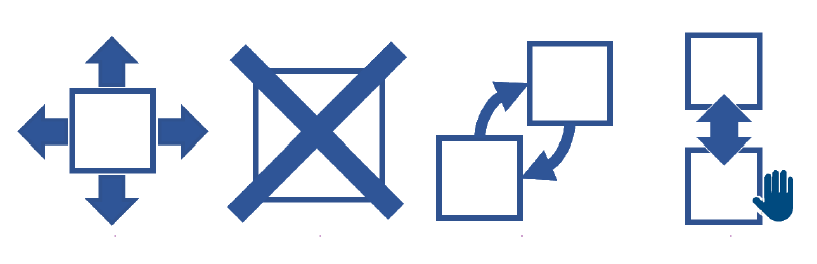
\includegraphics[width=0.6\textwidth]{image/Action tokens}
		\caption{Action tokens}
		\label{fig:action tokens}
	\end{figure}
	
\end{enumerate}

\subsubsection{Scoring Points}
In essence, scoring points has six combinations in this game. As you can see those combinations are under the table~\ref{tab:scoringPoints}. In each line, some combinations can appear simultaneously. Thus, the scoring points of a line depending on the combinations achieved in the respective line.

\begin{table}[h]
	\centering
	\begin{tabular}{|l|l|}
		\hline\xrowht[()]{10pt}
		Combinations          & Point    \\ 
		\hline\xrowht[()]{10pt}
		Six different symbols & 6 Points \\ 
		\hline\xrowht[()]{10pt}
		Two same symbols      & 1 Points \\
		\hline\xrowht[()]{10pt}
		Three same symbols    & 3 Points \\
		\hline\xrowht[()]{10pt}
		Four same symbols     & 5 Points \\ 
		\hline\xrowht[()]{10pt}
		Five same symbols     & 7 Points \\
		\hline
	\end{tabular}
	\renewcommand{\arraystretch}{4}
	\caption{A scoring points table.}
	\label{tab:scoringPoints}
\end{table}

\subsubsection{Player Mode}
This game has different player modes that can be only two players or four players to start a game. In addition, there are free combinations for each player that can be all human players, a mixture of human players and computer players, or all computer players. 

\subsubsection{The condition of winning a game}
There are two different approaches to reach winning a game. Generally speaking, the game should be ended when the game board is wholly occupied. However, if there is one team has completed six same tokens on a line on the chess board, then the game can be ended in advance and the winner appears. 

\begin{itemize}
	\item {Six same tokens}\\
    A team has arranged six same tokens on a board, then this team becomes the winner and the game is ended.
	
	\item {High Score}\\
    If there is no team that reaches six same tokens during the game, then scoring both teams at the end of the game. Which team has the higher score, the team is the winner. 
	
\end{itemize}

\subsection{Game Interface}

\subsubsection{Main Interface}

The main interface consists of several parts, a chess board, the area of players' hands, the display of the scoring combinations, the functional explanation of all action tokens, the demonstration of two team score points, and the label of the current player. 

\begin{enumerate}
	
	\item\textbf{Menu bar}\\
    In the main interface, the menu bar is apart into two separate sections. The first bar is called "setting", which obtains four menu items for the fundamental setting of the game, as Figure \ref{fig:settingMenu} below. 
	\begin{itemize}
		\item{Setting} \\ 
		\begin{itemize}
			\item {New Game} \\ 
		    The aims of the Menu item of New Game are used for creating a new game. 
			
			\item {Save} \\
			The aim of Menu item Save is used to save an incomplete game. The saving file is using GSON to translate the whole game system, including every player's state, the current board, the remained action tokens, and the current player.  
			
			\item {Load} \\
			The aim of Menu item Load is used to load a given game. A given file is provided with JSON and it can be analysed by using GSON to the whole game system, including every player's state, the current board, the remained action tokens, and the current player.  
			
			\item {Close} \\ 
			The function of Menu item Close is closing the game. 
			
		\end{itemize}
		
		
		\begin{figure}[h]
			\centering
			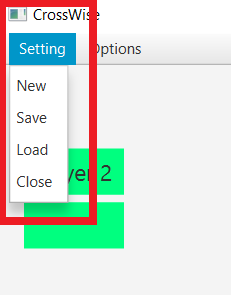
\includegraphics[width=0.3\textwidth]{image/settingMenu}
			\caption{The setting menu item}
			\label{fig:settingMenu}
		\end{figure}
		
		\newpage
		\item{Options} \\ 
		The options menu Figure \ref{fig:optionsMenu}  and explanation are shown below:
		\begin{itemize}
			\item {Duration} \\ 
			The menu item Duration contains three subdivisions, short, medium, and long, which are for dominating the duration of highlighting a cell on the chess board. 
			
			\item {Row/Column Score Display} \\
	    	The menu item Display Row/Column Score controls the visibility of seeing the score of each row and column. The default setting is invisible for all rows and columns.  
			
			\item {Current Team Points} \\
			The menu item Current Points controls the visibility of seeing the current total points of two teams. The default setting is invisible for the current team point.
			
			\item {Computer Hands} \\
			The menu item Computer Hands is utilized to manipulate the exhibition of the computer hands token. As there are bots participating in a game, the menu item could be executed for deciding whether their hands token should be visible or not. 
			
			\item {Stop AI playing} \\ 
	    	The menu item Stop AI Playing can be used to interrupt and cease the game when all players are a bot. The default setting is that this menu item is able implemented when all players are bots. 
			
		\end{itemize}
		
		\begin{figure}[h]
			\centering
			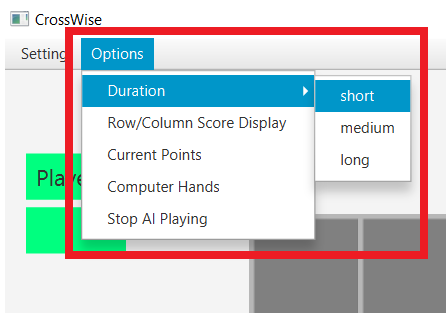
\includegraphics[width=0.5\textwidth]{image/OptionsMenu}
			\caption{The option menu}
			\label{fig:optionsMenu}
		\end{figure}
		
		
	\end{itemize}
	\newpage
\item\textbf{Chess board}\\
The chessboard is made of a 7x7-table, which is used for placing symbol tokens and displaying the score points of each line. Among, the 6x6-table where symbol tokens can be settled in each cell, is entirely occupied with a symbol token called None. Additionally, the endmost row and column remain empty in order to show the scoring point of each line. The graphic is shown below Figure \ref{fig:chessboard} .

\begin{figure}[h]
	\centering
	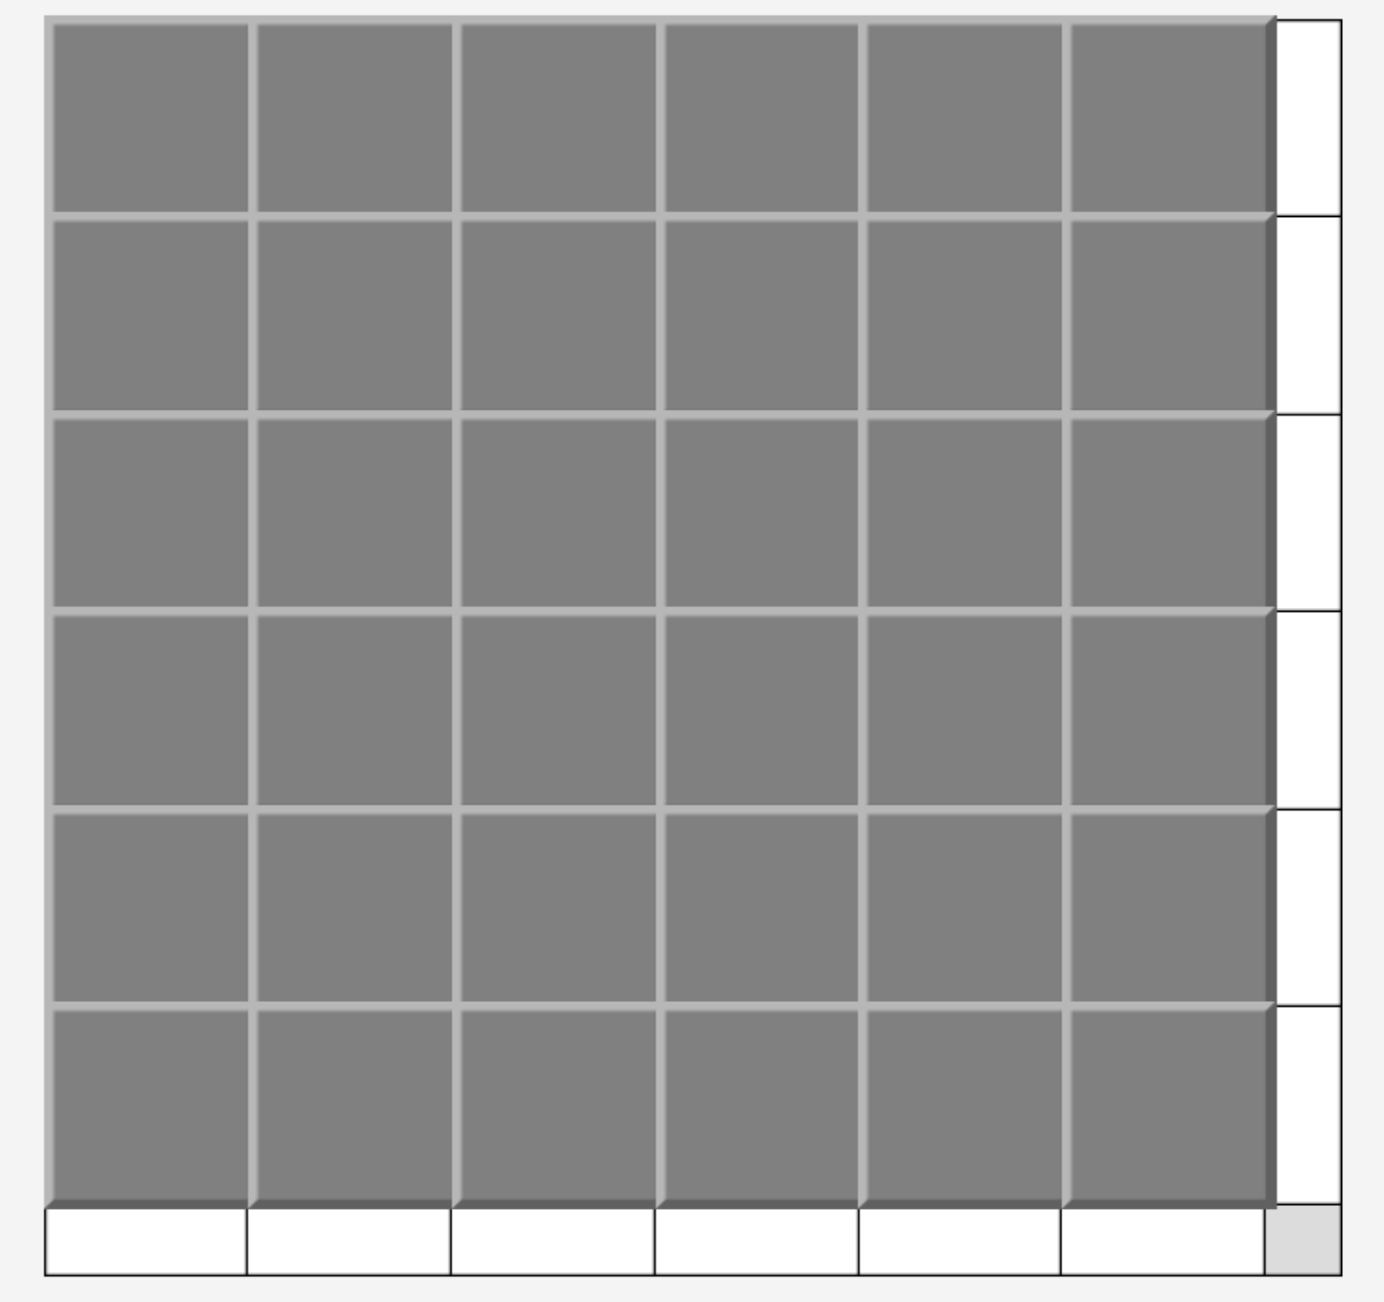
\includegraphics[width=0.6\textwidth]{image/chess board}
	\caption{The chess board}
	\label{fig:chessboard}
\end{figure}

\newpage
\item\textbf{Players' hands}\\ 
As shown in the Figure \ref{fig:playerhand} below, there are four red marking areas that surround the chess board, those areas are the players' hand tokens. 
If there are only two players involved in the game, then the exclusive area which is for player 1 and player 2 is visible..  

\begin{figure}[h]
	\centering
	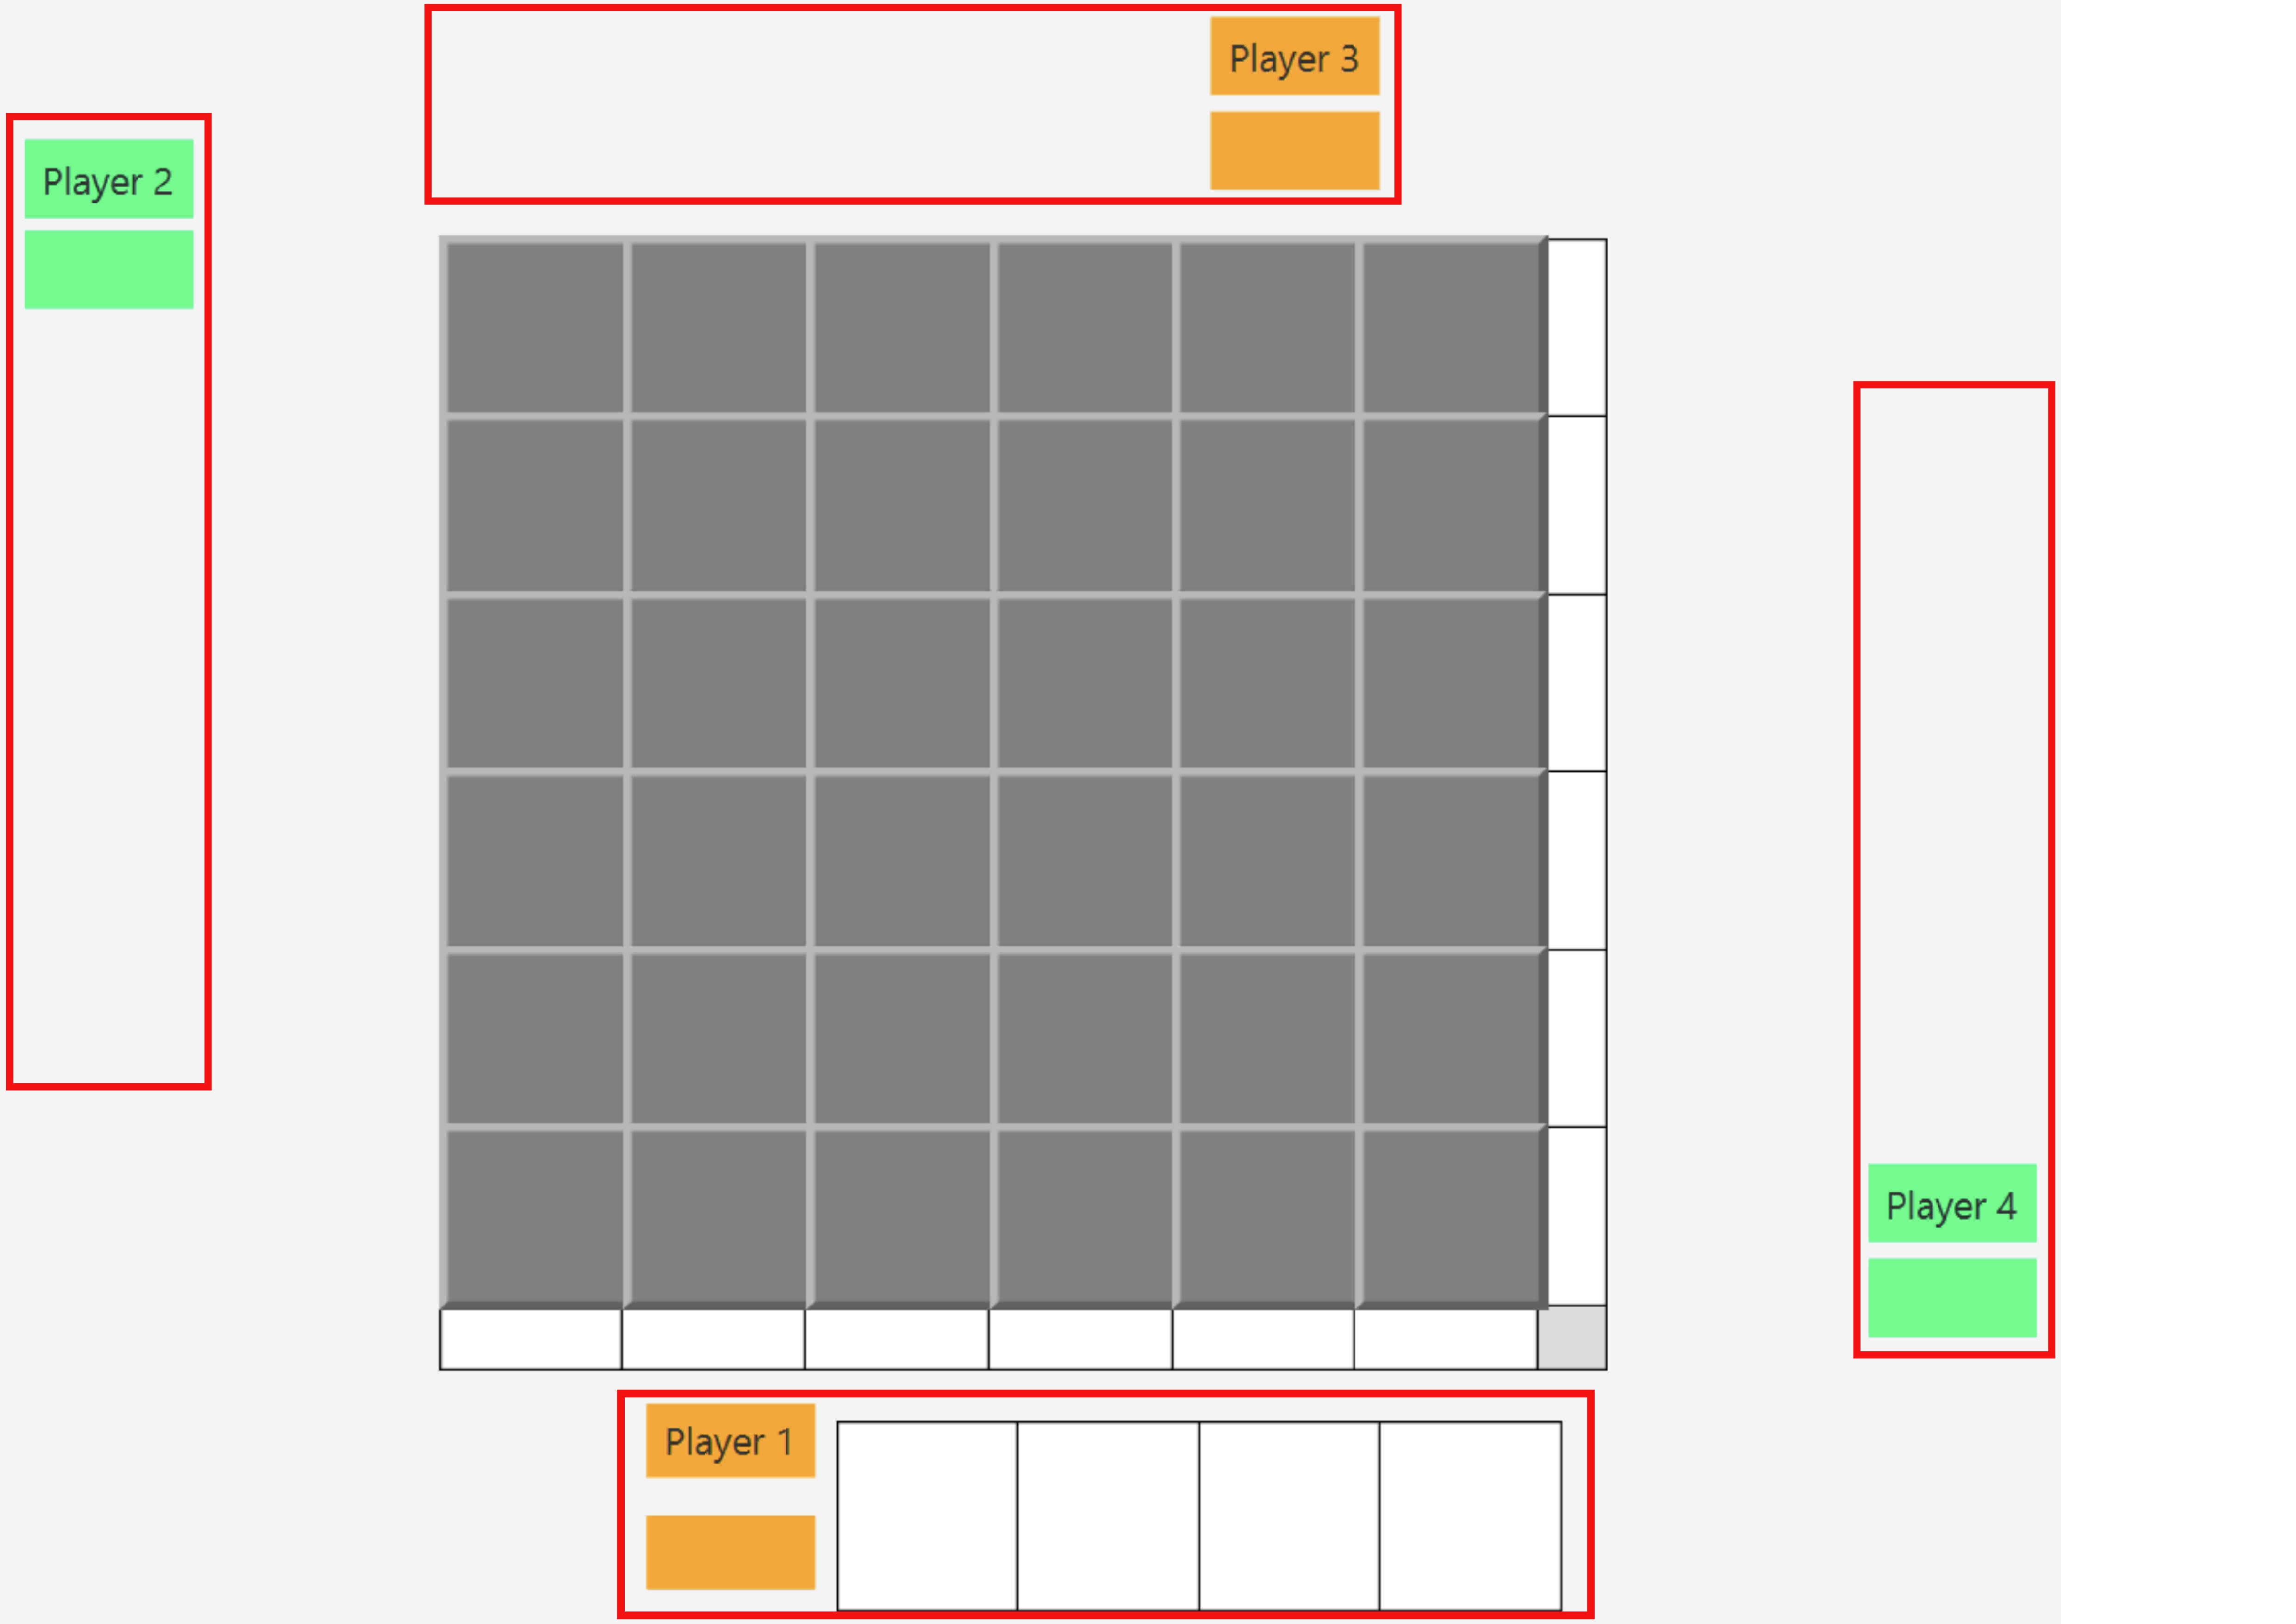
\includegraphics[width=0.8\textwidth]{image/players' hands }
	\caption{Players' hands}
	\label{fig:playerhand}
\end{figure}


\item\textbf{The combination of the scoring points }\\
On the right side of the main interface, a zone is for displaying all attainable combinations of every score. While the player is in the progress of the game, it is possibly forgotten how is the point being calculated. Hence, this region can remind players of the scoring logic. The demonstration is shown below in Figure \ref{fig:scoring points}.

\begin{figure}[h]
	\centering
	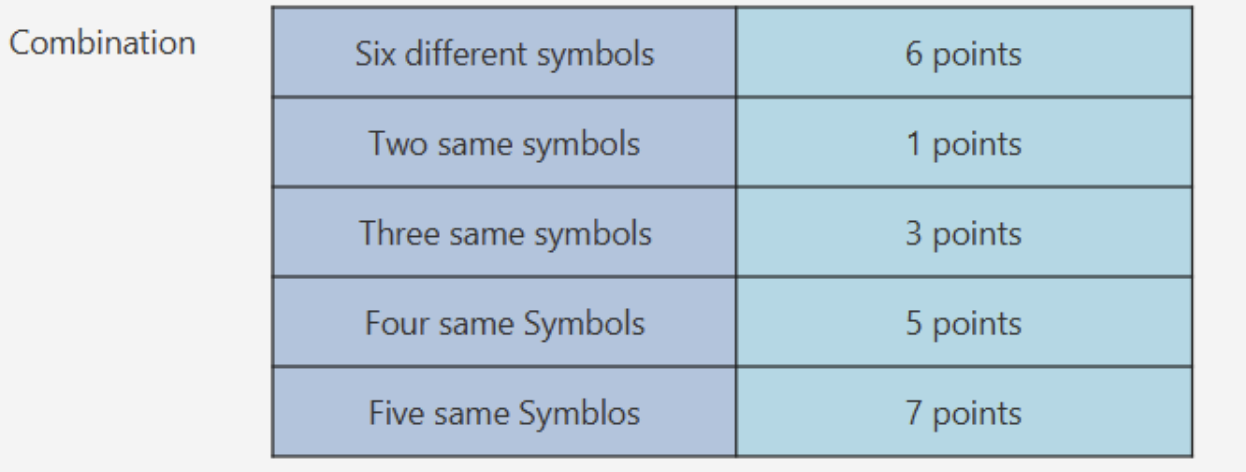
\includegraphics[width=0.8\textwidth]{image/scoring points}
	\caption{The combinations of scoring points}
	\label{fig:scoring points}
\end{figure}

\newpage

\item\textbf{The demonstration of two team score}\\
Undeniably, if the player can regularly inspect their current achievement, the experience of the game, and the convenience of the exploring game are increased undoubtedly. Therefore, possessing an area that demonstrates the achievement of two teams is a necessary arrangement. The demonstration is shown below in Figure \ref{fig:teamscore}.

\begin{figure}[h]
	\centering
	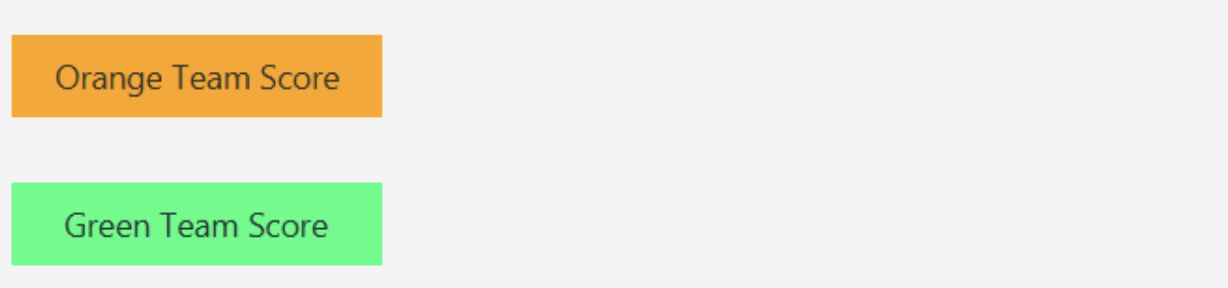
\includegraphics[width=0.8\textwidth]{image/two teams score}
	\caption{The display of team scores}
	\label{fig:teamscore}
\end{figure}

\item\textbf{The label of the current player}\\
As with the display of two team scores, labelling a current player is also an excellent option to enable participants to realize who turns. Meanwhile, the background colour of this label can be varied as the team belongs to the current player. The label is shown below in Figure \ref{fig:currentPlayer}.

\begin{figure}[h]
	\centering
	
\includegraphics[width=0.8\textwidth]{image/current Player}
	\caption{The label of current players}
	\label{fig:currentPlayer}
\end{figure}

\item\textbf{The explanation of all action tokens}\\
As with the same purpose of exhibiting combinations of the scoring points, having a description for action tokens provide considerable benefits for the game. Players can be reminded of the function of those four action tokens. 

Moreover, on the right side of the figure \ref{fig:the demonstration of action token} shown below, a list of the remaining number of action tokens is exhibited. Once one of these action tokens has been utilized, the list of the remaining number of action tokens will be updated automatically.  

\begin{figure}[h]
	\centering
	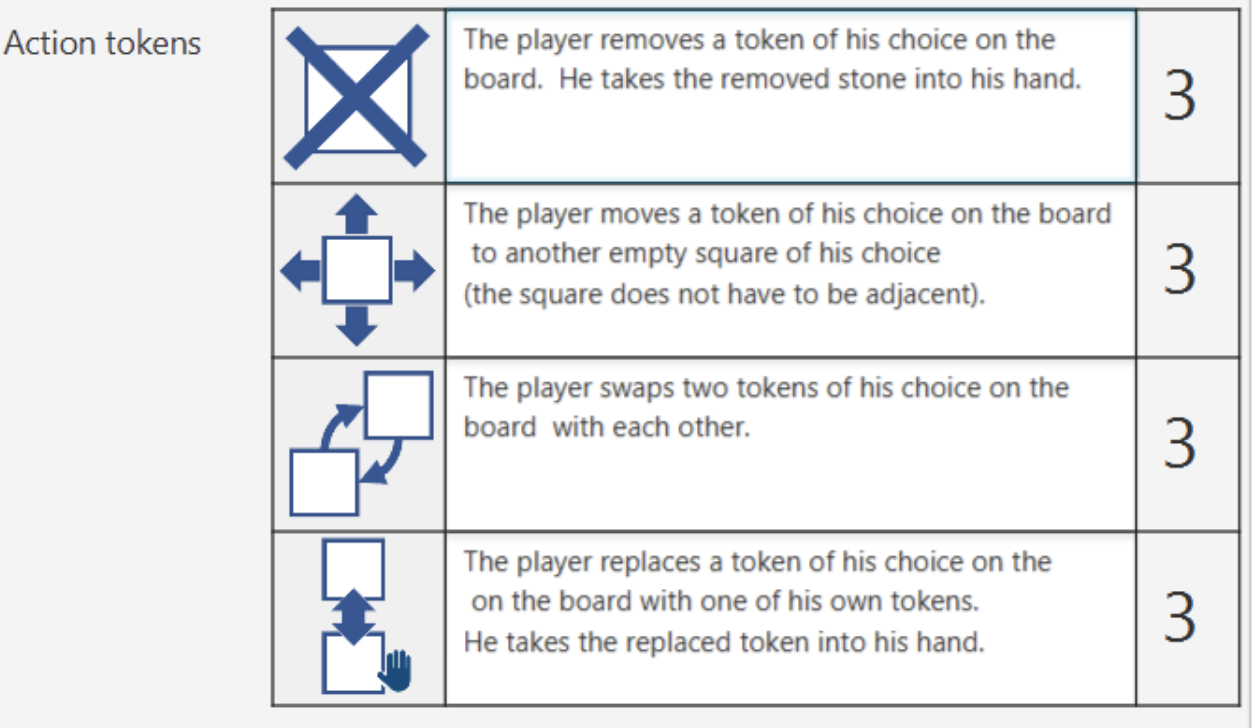
\includegraphics[width=0.6\textwidth]{image/the demonstration of Action token}
	\caption{The demonstration of action tokens}
	\label{fig:the demonstration of action token}
\end{figure}

\end{enumerate}

\newpage
\subsubsection{Secondary Interface}

\begin{enumerate}
	\item\textbf{Menu bar}\\
	The red marked area of the Figure \ref{fig:secondWindowMenu} represent the options menu items for deciding participants' number in a game. The default setting for initiating a game is four players.
	
	\begin{figure}[h]
		\centering
		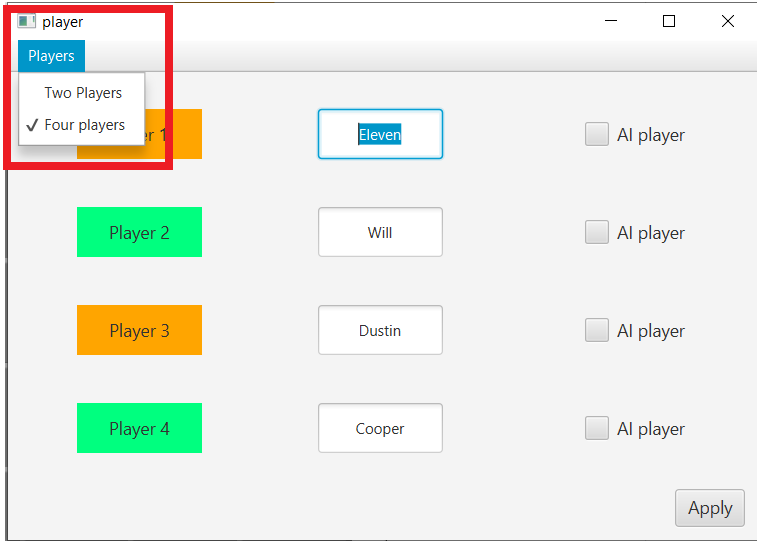
\includegraphics[width=0.6\textwidth]{image/secondWindowMenu}
		\caption{The menu bar in the second window}
		\label{fig:secondWindowMenu}
	\end{figure}
	
	
	
	\item\textbf{The second window}\\
	The Figure \ref{fig:playerScene} below represent an interface for initializing the state of players, involved in establishing player amounts, inputting players' name, and determining the state of the player in human or bot. As you can see the top-left corner has a menu item that can set up the number of players in a game. And in the middle of this scene which is circled as blue, there are four labels that can be entered players' names. At last, the right side of the scene which is marked as red provides four check boxes that enable the user to determine which players are manipulated by AI or humans.  
	
	\begin{figure}[h]
		\centering
		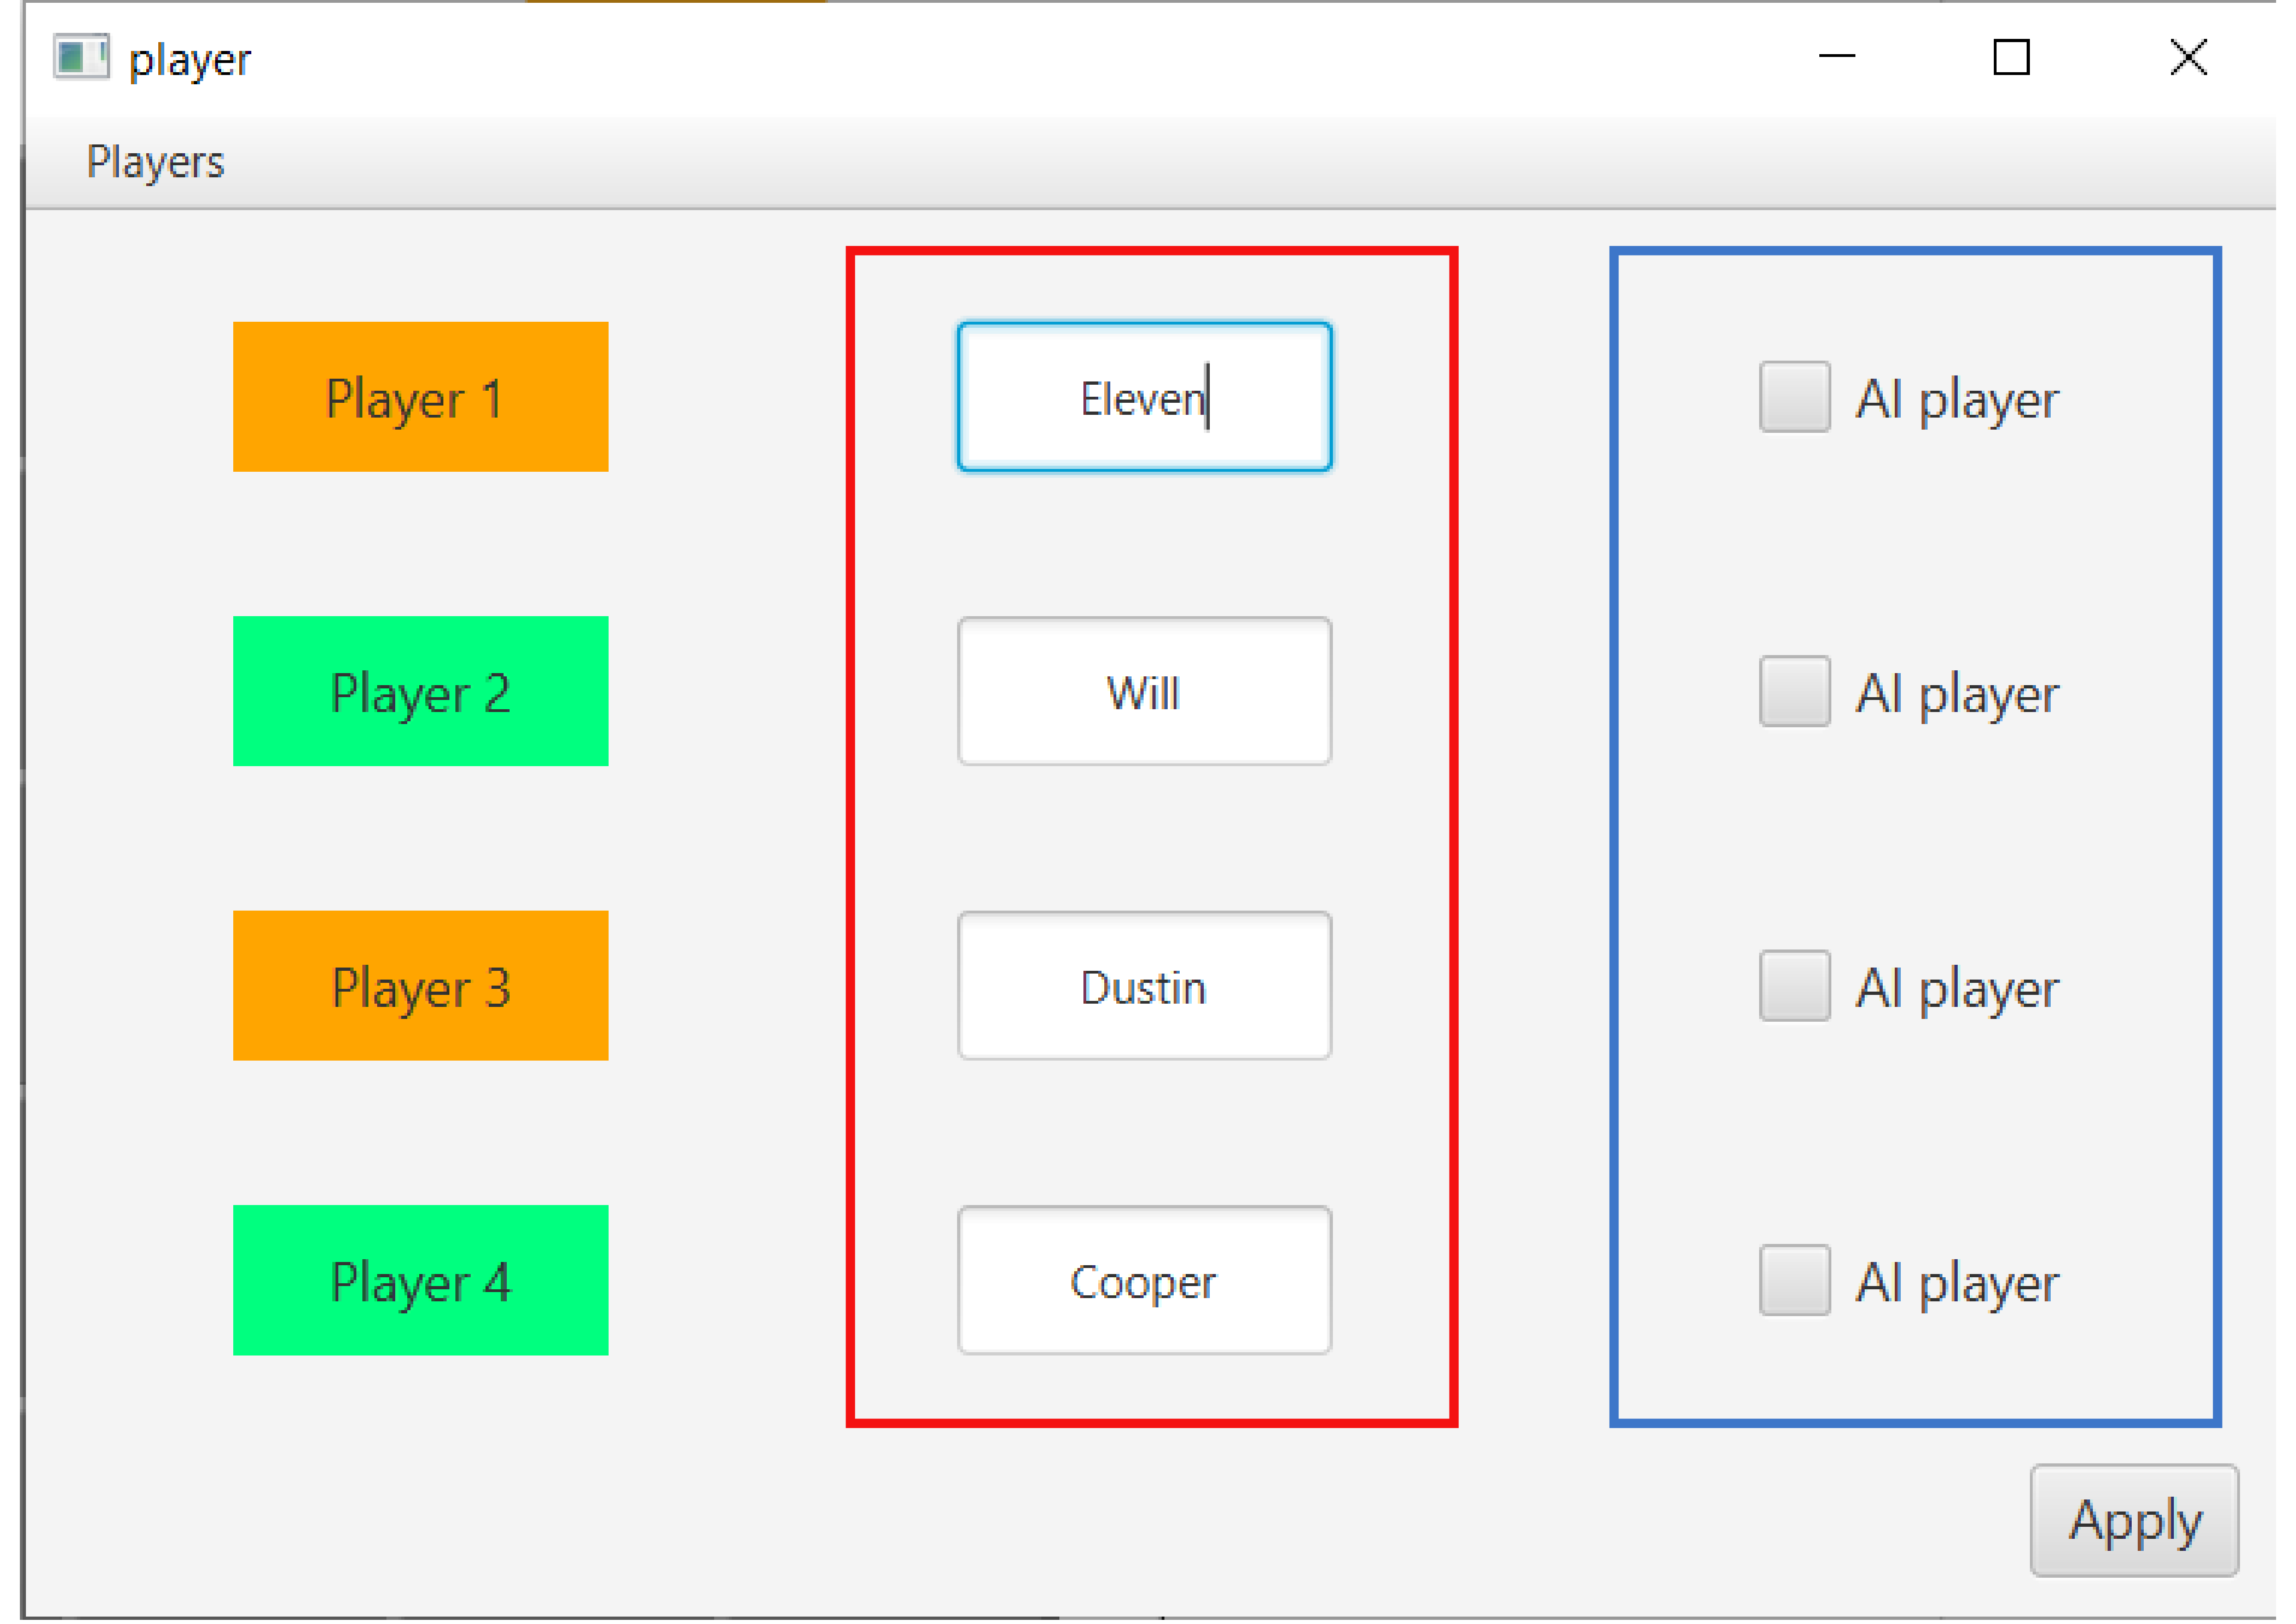
\includegraphics[width=0.6\textwidth]{image/Player scene}
		\caption{The second interface - player scene}
		\label{fig:playerScene}
	\end{figure}
\end{enumerate}

\newpage

\subsection{The Operation}

This paragraph is branched into three sections, before the beginning of the game, the game start, and the end of the game. 

\subsubsection{Before beginning of the game}
When the game is activated, a primary window is created and appeared, but the current interface cannot be clicked or manipulated by any action. Therefore, there are a few steps that can begin and activate a new game, which is shown below: 

\begin{enumerate}
	\item\textbf{The menu item "New Game"}\\
	The user should press the Menu Item "New Game" on the top-left corner to generate a new game.
	
	\item\textbf{Number of participants}\\
	Since the new game has been generated, a secondary scene which is for initiating player state arises. On the top-left corner of this secondary scene, the user can select the check menu Item to determine how many players should exist in a game. 
	
	\item\textbf{Inserting participants name and status}\\
    According to the selection of the number of participants, the user can insert every participant's name and decide which player is a bot or human.
	
	\item\textbf{Apply}\\
	At last, press the button, which is on the bottom-right corner to execute the game.
	
\end{enumerate}

\subsubsection{Game start}

\begin{enumerate}
	\item\textbf{A player's turn}\\
    During the game playing, one of the designs should be noticed that the game is being operated based on the turn of the current player. The hand token can be manipulated for the current player, nevertheless, other hand tokens are not allowed to give any movement or action.
	
	\item\textbf{Utilising tokens}\\
	Here have two different manipulative approaches for symbol tokens and action tokens. The instruction for two types of tokens is below:
	\begin{itemize}
		\item{Symbol token} \\
	    The manipulation behaviour of the symbol token is using drag and drop. The user needs to move their mouse on the symbol token of his or her hand token, which is chosen to move. And hold the left click and drag it to the chess board and release it on the desired cell of the chess board.  
		
		\item{Action token} \\
		The manipulative approach for using action tokens is clicking. Four action tokens use clicking action to activate the function of the action token. Firstly, as the user decides to use the action token, which is in his or her hand, it is simply a single click on the action token. However, the important and necessary noticed gist is that once the action token has been clicked, the user is not allowed to have other tokens chosen.  
		
		\begin{itemize}
			\item{Remove} \\
			The user should directly click on the desired cell of the chess board. Indeed, it is vital to realize that Remove is only allowing to click on the cell which has already occupied a token.  
			
			\item{Shifting} \\
	    	Based on the instruction of the shifting function, the user should select two positions on the board after clicking on the shifting token on their token hand. One is the position that contains a symbol token on a cell of the chess board and another should be an empty position which means no symbol token is placed.  
			
			\item{Exchange} \\
		    Regarding the function of the exchange token, the user has to choose two tokens on the chess board. After two tokens are selected by clicking, the animation of exchanging tokens is shown up to swap these two chosen tokens.  
			
			\item{Replace} \\
			Replace token has a unique function among these four action tokens. As the replace token has been activated, the user needs to select one symbol token on his or her hand before choosing another board token, which will be replaced.  
			Hence, if there is no other symbol token on the player's hand, then the Replace token cannot be executed.
			
		\end{itemize}
		
		
	\end{itemize}
	
	\item\textbf{Highlighting tokens}\\
	One design for raising up the game experience for players is that highlight every token, which is being dropped, clicked, or swapped. 
	Indeed, the token can be immediately and apparently noticed by highlighting after they are being changed position. 
	
\end{enumerate}

\newpage
\subsubsection{End the game}
Along with the game approaching the end and the winner is determined and appears, an alert message has emerged with a window like a Figure \ref{fig:winnerMessage} below. The message shows which team is winning the game and also the reason for winning the game.  

However, once the message is read and closed, the main interface becomes disabled to access or manipulate until the user selects a new game on the menu item.  

\begin{figure}[h]
	\centering
	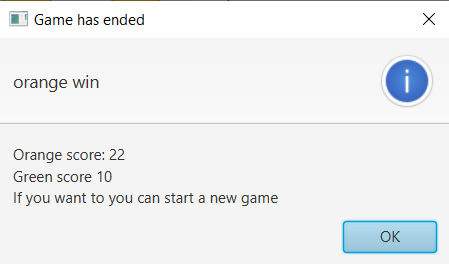
\includegraphics[width=0.5\textwidth]{image/winner message}
	\caption{The winning message}
	\label{fig:winnerMessage}
\end{figure}




\newpage
\section{Error messages}


\subsection{During the game}

\begin{table}[h]
	\centering
\begin{tabular}{p{2.5cm}@{\hskip 5mm}  p{5cm}@{\hskip 5mm} p{6.5cm}} 
	\toprule
	error message   & cause      & corrective action  \\ 
	\midrule
	\midrule
    Exchange token cannot be used & Player may not use Exchange Token when there are less than two tokens on the board & Reselect an available token on his hand  \\

	\bottomrule
\end{tabular}
\end{table}

\begin{figure}[h]
	\centering
	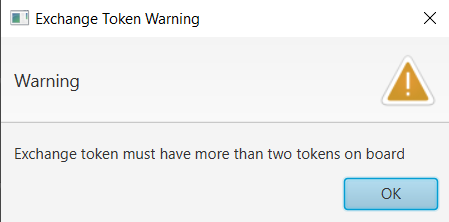
\includegraphics[width=0.6\textwidth]{image/ExchangeToken}
	\caption{Exchange Token Warning}
	\label{fig:ExchangeTokenWarning}
\end{figure}

\newpage

\subsection{Load and Save}


\begin{table}[h]
	\centering
	\begin{tabular}{p{2.5cm}@{\hskip 5mm}  p{5cm}@{\hskip 5mm} p{6.5cm}} 
		\toprule
		error message   & cause      & corrective action  \\ 
		\midrule
		\midrule
     	The chosen file does not exist & There is no file selected to load and the file for saving does not input the file name & Press Load/Save Menu Item again and re-selected a file  \\
	    \midrule
	    The player amount is not correct & If the input file contains an invalid player amount, it causes the incorrect execution of the game. & Check the format of the input file and reload again. \\

		\bottomrule
	\end{tabular}
\end{table}

\begin{figure}[h]
	\centering
	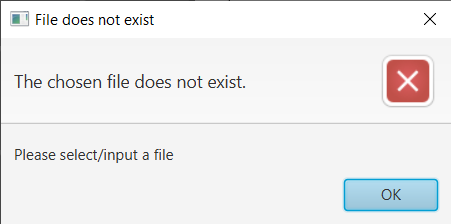
\includegraphics[width=0.6\textwidth]{image/SaveAndLoad}
	\caption{The chosen file is not exist}
	\label{fig:The chosen file does not exist}
\end{figure}

\begin{figure}[h]
	\centering
	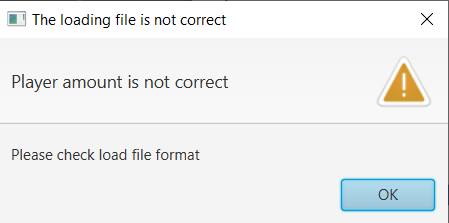
\includegraphics[width=0.6\textwidth]{image/alertPlayerAmount}
	\caption{The alert of wrong player amount}
	\label{fig:The alert of wrong player amount}
\end{figure}

\newpage

\subsection{Stop AI running}

\begin{table}[h]
	\centering
\begin{tabular}{p{2.5cm}@{\hskip 5mm}  p{5cm}@{\hskip 5mm} p{6.5cm}} 
		\toprule
		error message   & cause      & corrective action  \\ 
		\midrule
		\midrule
	    Stop AI Running & A radio button is pressed and it can terminate the JavaFX Program  &  Following the instruction given in the window. Press the New game button to start a new game \\ 
		\bottomrule
	\end{tabular}
\end{table}

\begin{figure}[h]
	\centering
	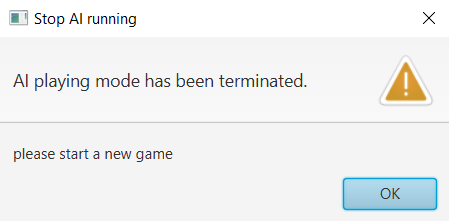
\includegraphics[width=0.6\textwidth]{image/StopAIRunning}
	\caption{Terminate AI Running}
	\label{fig:Terminate AI Running}
\end{figure}

\newpage

\subsection{No available hand token}

\begin{table}[h]
	\centering
	\begin{tabular}{p{2.5cm}@{\hskip 5mm}  p{5cm}@{\hskip 5mm} p{6.5cm}} 
		\toprule
		error message   & cause      & corrective action  \\ 
		\midrule
		\midrule
		Full of action token and the chessboard has no token  & If the player has all action tokens on hand, meanwhile the board is empty without any symbole token to allow action token to implement its function &  This game needs to be restart by clicking New Game button  \\
		\midrule
		Full of Replace Token and No symbol Token  & If the player has clicked their token hand, which contains three replace tokens and no symbol tokens, the game cannot be continuously played.  &  The game should be restarted by clicking the New Game button on the top left.  \\
		\bottomrule
	\end{tabular}
\end{table}

\begin{figure}[h]
	\centering
	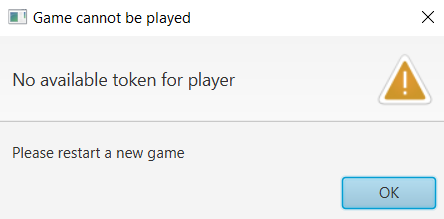
\includegraphics[width=0.6\textwidth]{image/NoToken}
	\caption{No available token hand}
	\label{fig:No available token hand}
\end{figure}